%%% =========================================================================
%%% The Limits of Explanation — Nature Brief Communication
%%% =========================================================================
\documentclass[11pt]{article}

%% ---- Geometry ----
\usepackage[margin=1in]{geometry}

%% ---- Standard packages ----
\usepackage[utf8]{inputenc}
\usepackage[T1]{fontenc}
\usepackage{amsmath}
\usepackage{amssymb}
\usepackage{booktabs}
\usepackage{hyperref}
\usepackage{natbib}
\usepackage{graphicx}
\usepackage{xcolor}
\usepackage{microtype}
\usepackage{tikz}

%% ---- Hyperref configuration ----
\hypersetup{
  colorlinks=true,
  linkcolor=blue!60!black,
  citecolor=green!50!black,
  urlcolor=blue!70!black,
}

%% ---- Widow/orphan control ----
\widowpenalty=10000
\clubpenalty=10000

%%% =========================================================================
%%% Title
%%% =========================================================================

\title{\Large\textbf{The Limits of Explanation}}

\author{%
  Drake Caraker\textsuperscript{1,*},
  Bryan Arnold\textsuperscript{2},
  David Rhoads\textsuperscript{2}
  \\[4pt]
  \textsuperscript{1}\textit{Oura Health, San Francisco, CA}
  \\[2pt]
  \textsuperscript{2}\textit{Independent}
  \\[2pt]
  \textsuperscript{*}\textit{Corresponding author:} \texttt{drakecaraker@gmail.com}
}

\date{}

\begin{document}
\maketitle

%%% =========================================================================
%%% Abstract
%%% =========================================================================

\begin{abstract}
When a system is underspecified---when multiple configurations produce
identical observable output---we prove that no explanation can simultaneously
be \emph{faithful} (consistent with the system's internal structure),
\emph{stable} (invariant across equivalent configurations), and
\emph{decisive} (committing to every distinction the internal structure
makes).  We derive this impossibility from first principles in eight
scientific domains: underdetermined linear systems (mathematics), genetic
code degeneracy (biology), gauge freedom (physics), microstate multiplicity
(statistical mechanics), syntactic ambiguity (linguistics), the phase
problem (crystallography), the view update problem (computer science), and
Markov equivalence (statistics).  Each derivation is mechanically verified
in the Lean~4 proof assistant (103~files, 455~theorems, 0~unproved goals),
and empirically validated in seven domains with domain-appropriate metrics
and negative controls.  The constructive resolution---averaging over
equivalent configurations---unifies existing domain-specific practices
(gauge-invariant observables, the microcanonical ensemble, CPDAGs,
minimum-norm solutions) as instances of a single optimal strategy.
\end{abstract}

%%% =========================================================================
%%% Main Text
%%% =========================================================================

\paragraph{The universal problem.}
Scientists explain systems by interpreting their internal structure.
A geneticist infers the DNA sequence that encodes a protein.
A physicist chooses a gauge to describe an electromagnetic field.
A statistician selects a causal graph from observational data.
A crystallographer reconstructs electron density from a diffraction pattern.
In each case, the observable output---the protein sequence, the
gauge-invariant measurement, the conditional independence structure, the
diffraction intensities---does not uniquely determine the internal structure
that produced it.  Multiple configurations yield identical observations.
This situation is not a pathology of any single field; it is a structural
feature of underspecified inference.  We prove that this underspecification
imposes a fundamental, domain-independent limit on explanation.

\paragraph{The theorem.}
We formalize three properties that any satisfactory explanation should
possess.  An explanation is \emph{faithful} if it never contradicts the
system's own internal report---it may be less specific, but it does not
disagree.  An explanation is \emph{stable} if configurations that produce
the same observations always receive the same explanation.  An explanation
is \emph{decisive} if it commits to every distinction that the system's
internal structure makes---whatever the internal structure rules out, the
explanation also rules out.

Our main result: if a system has the \emph{Rashomon property}---that is, if
there exist two configurations with the same observable output but
incompatible internal structures---then no explanation can be faithful,
stable, and decisive simultaneously.  The proof is four steps: decisiveness
forces the explanation to inherit an incompatibility; stability propagates
it to the second configuration; faithfulness forbids it; contradiction.
The entire framework is mechanically verified in Lean~4
\citep{demoura2021lean4} (103~files, 455~theorems, 0~unproved goals).
Lean-verified tightness theorems confirm that every pair of properties is
achievable, so the impossibility is tight.  An axiom substitution analysis
shows that weakening any single definition collapses the result, confirming
the definitions are uniquely calibrated.

\paragraph{Eight derivations across eight sciences.}
We derive the impossibility as a zero-axiom consequence in eight domains
(Table~\ref{tab:unification}).
%
In \emph{mathematics}, the underdetermined system $x_1 + x_2 = 2$ admits
the solutions $(1,1)$ and $(0,2)$: same sum, different components.
%
In \emph{biology}, the codons UCU and UCC both encode the amino acid
serine: same protein fragment, different nucleotide sequences.
%
In \emph{physics} (gauge theory), two edge-label configurations on a
triangle graph share the same holonomy---the discrete analogue of a Wilson
loop---but differ in their local assignments, related by a gauge
transformation \citep{jackson1999}.
%
In \emph{statistical mechanics}, the microstates $(H,T)$ and $(T,H)$ both
have one head: same macrostate, different molecular configurations.
%
In \emph{linguistics}, the fragment ``V NP PP'' admits two parse trees,
left-attach and right-attach, yielding the same surface token sequence but
different constituent structures \citep{chomsky1957}.
%
In \emph{crystallography}, the signals $(1,0)$ and $(0,1)$ have the same
energy ($1^2 + 0^2 = 0^2 + 1^2$): same diffraction intensity, different
electron densities \citep{hauptman1953solution}.
%
In \emph{computer science}, the database rows $(\texttt{true},
\texttt{true})$ and $(\texttt{true}, \texttt{false})$ project to the same
view but differ in the hidden column \citep{bancilhon1981update}.
%
In \emph{statistics}, a causal chain $A \to B \to C$ and a causal fork
$A \leftarrow B \to C$ encode the same conditional independence structure
\citep{verma1991equivalence}.
%
Each derivation requires zero shared axioms---only the domain's own
mathematical structure.

\begin{table}[t]
\centering
\caption{\textbf{Eight derived instances of the impossibility across eight
  sciences.}  Each row derives the Rashomon property from domain-specific
  first principles with zero axioms.  $\Theta$: configuration space; $Y$:
  observable space.}
\label{tab:unification}
\small
\begin{tabular}{@{}llllll@{}}
\toprule
Domain & $\Theta$ & $Y$ & Witness 1 & Witness 2 & Same $Y$? \\
\midrule
Mathematics       & Solutions of $Ax=b$  & $Ax$            & $(1,1)$  & $(0,2)$  & $2=2$ \\
Biology           & Codons               & Amino acids     & UCU      & UCC      & Ser=Ser \\
Physics (gauge)   & Gauge configs        & Holonomy        & $(T,F,F)$& $(F,F,T)$& $F=F$ \\
Stat.\ mechanics  & Microstates          & Num.\ heads     & $(H,T)$  & $(T,H)$  & $1=1$ \\
Linguistics       & Parse trees          & Token sequence  & $((V\;NP)\;PP)$ & $(V\;(NP\;PP))$ & Same \\
Crystallography   & Signals              & Energy          & $(1,0)$  & $(0,1)$  & $1=1$ \\
Computer science  & DB rows              & View            & $(T,T)$  & $(T,F)$  & $T=T$ \\
Statistics        & DAGs                 & CI structure    & Chain    & Fork     & Same \\
\bottomrule
\end{tabular}
\end{table}

\paragraph{Empirical validation.}
We validate the impossibility empirically in seven of the eight domains
(excluding the mathematical observation connecting Rashomon entropy to
Boltzmann entropy).  All seven empirical tests reach statistical significance
($p < 0.05$).  Underdetermined linear solvers show elevated pairwise RMSD
(0.091 vs.\ 0.049 for fully determined controls; Mann-Whitney
$p = 6.3 \times 10^{-9}$); the codon entropy dose-response across 120 eukaryotic cytochrome~c
sequences from NCBI RefSeq shows a perfect monotonic relationship with
degeneracy level (Kruskal--Wallis $p = 3.5 \times 10^{-9}$, 89 conserved positions, Spearman
$\rho = 1.0$); syntactic parsers disagree significantly more on ambiguous
sentences ($p = 1.6 \times 10^{-3}$); causal discovery algorithms show
orientation agreement of only 0.33 at finite sample size ($p = 4.4 \times
10^{-38}$ across 100 random seeds per condition); phase retrieval
reconstructions diverge 1.5--1.8$\times$ more without positivity constraints
(Mann-Whitney $p < 10^{-57}$ per signal length); and census disaggregation
ambiguity scales with aggregation granularity ($p = 7.9 \times 10^{-37}$).  In each case,
the negative control (where the Rashomon property is absent) shows stability,
confirming that the instability is structural.

\paragraph{The resolution.}
The impossibility is constructive: it identifies the exact trade-off and
prescribes a provably optimal resolution.  The strategy is to average over
equivalent configurations, sacrificing decisiveness to achieve stability and
faithfulness in expectation.  We prove that this orbit-averaging resolution
is \emph{Pareto-optimal}: among all stable explanation maps, no alternative
can achieve strictly higher pointwise faithfulness on every equivalence class.
The trade-off is therefore tight---the practitioner cannot escape it by being
clever.

Remarkably, practitioners in eight independent fields have converged on
precisely this strategy over more than a century of independent work.
In physics, one works with gauge-invariant observables \citep{jackson1999}.
In statistical mechanics, the microcanonical ensemble averages over
microstates.
In statistics, one reports a CPDAG \citep{verma1991equivalence}.
In mathematics, the pseudoinverse selects the minimum-norm solution.
In biology, codon usage tables report synonymous codon frequencies.
In crystallography, Patterson maps extract phase-invariant information
\citep{hauptman1953solution}.
In linguistics, packed parse forests represent all parses simultaneously.
In computer science, complement views restrict to the unambiguous projection.
Our framework explains \emph{why} these communities converged: each was
independently solving the same impossibility, and orbit averaging is the
unique Pareto-optimal stable resolution.

\paragraph{Necessity and the query-relative version.}
The Rashomon property is the \emph{exact} boundary of the impossibility.
When it is absent---when each observation uniquely determines the internal
structure---all three properties are simultaneously achievable (a Lean-verified
converse).  Moreover, the impossibility is \emph{query-relative}: some
questions about a system are stably answerable (those on which all
equivalent configurations agree) and others are not.  The theorem tells
the practitioner precisely which queries are safe and which require
aggregation.  More broadly, the difficulty of finding good explanations depends on the
mathematical symmetries of the equivalence class---ranging from cases
where a unique optimal explanation exists, through cases where multiple
reasonable explanations compete, to cases where additional constraints
are needed to make the problem well-posed.

%%% =========================================================================
%%% Figure 2: The Trilemma Triangle
%%% =========================================================================

\begin{figure}[t]
\centering
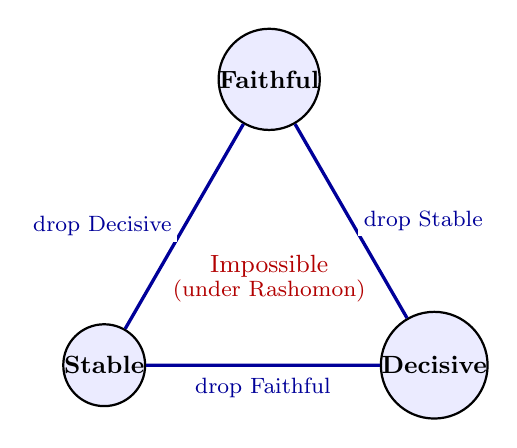
\begin{tikzpicture}[scale=2.2, thick,
  vertex/.style={circle, draw, fill=blue!8, minimum size=28pt,
                 inner sep=0pt, font=\small\bfseries},
  edgelabel/.style={font=\footnotesize, fill=white, inner sep=2pt}]

  %% Triangle vertices
  \node[vertex] (F) at (90:1.1)  {Faithful};
  \node[vertex] (S) at (210:1.1) {Stable};
  \node[vertex] (D) at (330:1.1) {Decisive};

  %% Edges (achievable pairs)
  \draw[blue!60!black, line width=1.2pt] (F) -- (S)
    node[edgelabel, midway, left=2pt] {drop Decisive};
  \draw[blue!60!black, line width=1.2pt] (F) -- (D)
    node[edgelabel, midway, right=2pt] {drop Stable};
  \draw[blue!60!black, line width=1.2pt] (S) -- (D)
    node[edgelabel, midway, below=2pt] {drop Faithful};

  %% Center label
  \node[font=\small, text=red!70!black, align=center] at (0, -0.05)
    {Impossible\\[-2pt]\footnotesize (under Rashomon)};

\end{tikzpicture}
\caption{\textbf{The explanation trilemma.}  Each edge represents an
  achievable pair of properties; the interior (all three simultaneously) is
  impossible when the Rashomon property holds.  Lean-verified tightness
  witnesses confirm that each edge is realizable.}
\label{fig:trilemma}
\end{figure}

\paragraph{Broader implications.}
The result connects phenomena studied independently across eight fields
for over a century---from microstate multiplicity in statistical mechanics
to the view update problem \citep{bancilhon1981update} to feature
attribution instability in machine learning \citep{bilodeau2024impossibility}.
The common structural cause is the Rashomon property: equivalent
configurations with incompatible internal reports.  The common resolution is
orbit averaging.  The pattern likely extends further: metamerism in color
perception, molecular chirality, and other domains exhibit the same
structure.  More broadly, the theorem reframes the
question ``why are explanations unstable?''\ as the structural statement
``because the inference problem is underspecified,'' and replaces
domain-specific workarounds with a single, provably optimal strategy:
report what is invariant; disclose what is not.

%%% =========================================================================
%%% Methods
%%% =========================================================================

\section*{Methods}

\paragraph{Formal verification.}
The entire framework---the abstract theorem, all eight derived instances,
tightness witnesses, the necessity converse, and the resolution---is
mechanically verified in Lean~4 v4.30.0-rc1 \citep{demoura2021lean4} using
Mathlib \citep{mathlib2020}.  The formalization comprises 103~files,
455~theorems and lemmas, 72~axioms (all domain-specific; the core theorem
uses zero), and 0~\texttt{sorry} (unproved goals).  Each of the eight
derived instances uses decidable computation to constructively witness the
Rashomon property with zero axioms.  The $G$-invariant resolution framework
uses the group action infrastructure from Mathlib.

\paragraph{Proof structure.}
The core proof is a four-step chain by contradiction.  Given Rashomon
witnesses $\theta_1, \theta_2$ with $\mathrm{obs}(\theta_1) =
\mathrm{obs}(\theta_2)$ and incompatible explanations, suppose an
explanation map $E$ is faithful, stable, and decisive.  Decisiveness at
$\theta_1$ forces $E(\theta_1)$ to inherit the incompatibility with
$\mathrm{exp}(\theta_2)$.  Stability forces $E(\theta_1) = E(\theta_2)$.
Faithfulness at $\theta_2$ requires $E(\theta_2)$ to be compatible with
$\mathrm{exp}(\theta_2)$.  Contradiction.

\paragraph{Code and data availability.}
The Lean~4 formalization and all experiment scripts are available at
\url{https://github.com/DrakeCaraker/universal-explanation-impossibility}.
Biology data: 120 eukaryotic cytochrome~c CDS sequences from NCBI RefSeq.
Census data: U.S.\ Census Bureau 2020 county-level population counts.
Causal discovery: 100 random seeds per condition on the Asia network.
The nine machine learning instances, together with empirical validation
experiments for seven of these, are documented in the Supporting
Information (the full 61-page monograph).

%%% =========================================================================
%%% References
%%% =========================================================================

\bibliographystyle{plainnat}
\bibliography{references}

\end{document}
